

\documentclass[fontsize=12pt]{article}
\usepackage{fourier}
%%% Custom sectioning
\usepackage{sectsty}
\allsectionsfont{\flushleft \normalfont\scshape}
\usepackage[font=scriptsize,labelfont=bf]{caption}
\usepackage[english]{babel}															% English language/hyphenation
\usepackage[protrusion=true,expansion=true]{microtype}	
\usepackage{amsmath,amsfonts,amsthm} % Math packages
\usepackage[pdftex]{graphicx}	

\usepackage{url}
\usepackage[margin=1 in]{geometry}
\geometry{a4paper}

\usepackage{graphicx}
\usepackage{listings}
\usepackage{float}
\usepackage{xcolor}
% page counting, header/footer
\usepackage{fancyhdr}
\usepackage{lastpage}
\pagestyle{fancy}
\lhead{\footnotesize \parbox{11cm}{Office Object Recognition} }
%\renewcommand{\headheight}{24pt}


\begin{document}

\begin{titlepage}

\newcommand{\HRule}{\rule{\linewidth}{0.5mm}} % Defines a new command for the horizontal lines, change thickness here

\center % Center everything on the page
 
%----------------------------------------------------------------------------------------
%	HEADING SECTIONS
%----------------------------------------------------------------------------------------

\textsc{\LARGE Erasmus Mundus Master in Vision and Robotics}\\[1.5cm] % Name of your university/college
\textsc{\Large B31XP:Robotics Project }\\[0.5cm] % Major heading such as course name
%\textsc{\large Minor Heading}\\[0.5cm] % Minor heading such as course title

%----------------------------------------------------------------------------------------
%	TITLE SECTION
%----------------------------------------------------------------------------------------

\HRule \\[0.4cm]
{ \huge \bfseries Office Object Recognition}\\[0.4cm] % Title of your document
\HRule \\[1.5cm]
 
%----------------------------------------------------------------------------------------
%	AUTHOR SECTION
%----------------------------------------------------------------------------------------

\begin{minipage}{0.4\textwidth}
\begin{flushleft} \large
\emph{Los Lobos Solitarios v2.0}\\
Abraham \textsc{Ayala} \\% Your name
Quim \textsc{Sanchez}\\ % Your name
Waldemar \textsc{Franczak}\\ % Your name
\end{flushleft}
\end{minipage}
~
\begin{minipage}{0.4\textwidth}
\begin{flushright} \large
\emph{Supervisor:} \\
Dr. Zeyn \textsc{Saigol} % Supervisor's Name
\end{flushright}
\end{minipage}\\[4cm]

% If you don't want a supervisor, uncomment the two lines below and remove the section above
%\Large \emph{Author:}\\
%John \textsc{Smith}\\[3cm] % Your name

%----------------------------------------------------------------------------------------
%	DATE SECTION
%----------------------------------------------------------------------------------------

{\large \today}\\[3cm] % Date, change the \today to a set date if you want to be precise

%----------------------------------------------------------------------------------------
%	LOGO SECTION
%----------------------------------------------------------------------------------------

%\includegraphics{Logo}\\[1cm] % Include a department/university logo - this will require the graphicx package
 
%----------------------------------------------------------------------------------------

\vfill % Fill the rest of the page with whitespace

\end{titlepage}
\tableofcontents
\pagebreak[4]
\section{Introduction}\label{sec:intro}
This report describes the advances done by Lobos Solitarios v 2.0 team in the Office Object Recognition project. The general goal of the project is to implement a pipeline which provides an ability for a mobile robot to perform object recognition of objects commonly present in office environments. Such information might be useful in order to provide environmental awareness and allow robots to perform more advanced and useful tasks. Due to the popularity and increase in the use of mobile robots, a convenient area of research is the recognition of objects present in office environments, since it is easy to have access to chairs, tables, stools, etc. For this reason the project described in this report will focus on the recognition problem of common office objects like chairs and tables. The solution developed can be extended to other type of scenes like factories, schools, outdoors, etc.  \\ \linebreak
This work is organized as follows, in section \ref{sec:toolseval} the requirements and initial goals of the project will be described as well the evaluation of the initial proposed tools. In section \ref{sec:planning}  the project planning which describes how the time was administrated and the changes in the planning will be discussed. In sections \ref{sec:map} through \ref{sec:recognition} the proposed solution of the team is explained. Finally in section \ref{sec:Future Work} the future work to be done and conclusions are  derived. 
\section{Requirements and Evaluation of Tools}
 \label{sec:toolseval}
The developed solution to address the problem of common office object recognition should meet several conditions described below.\\
Preferably the system should be able to recognize the objects even though the object is partially occluded or only part of its components are seen. To achieve this, a possible solution is to define object classes which are composed by different elements. For example a chair is composed by subcomponents as shown in figure \ref{fig:chair}; in some situations it is possible that the robot only observes one or several of these subcomponents of the class chair. The system should be able to recognize or give probabilities of how likely is a set of structural elements to form an object class.

\begin{figure}[H]
\begin{center}
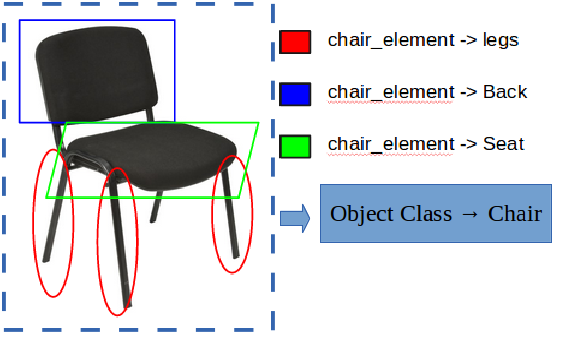
\includegraphics[width=0.5\linewidth]{images/chair}
\caption{Decomposition of the class 'chair' into its structural elements}
\label{fig:chair}
\end{center}
\end{figure}
It is important to denote that since the robot will be moving, the scale of the objects observed can change, this should be taken into account when developing the recognition algorithm.
In a more advanced phase of the project, is intended to provide the robot the ability to identify when an object is incomplete, this with the purpose of moving it to the unknown part of the object and fuse the information of different views. 
The development of the whole project implies a challenging problem and is the subject of current research \cite{bib:semantic}. The output of this project provides an initial framework for solving the problem, and will be a basis for future VIBOT projects \\

The available hardware platform for this phase of the project is:
\begin{itemize}
\item Turtlebot 2 mobile robot from willow garage and clearpath, which is equipped with two motorized wheels and two non motorized supporting wheels. Some platforms and supports are available to hold extra sensors, CPU, tools, etc. 
\item Microsoft Kinect  1 (640x480) RGB-D system fixed to turtlebot's chassis. This will be the sensing element to obtain 3D and RGB information of the scene. 
\end{itemize}
In terms of software tools, the desired or preferable platforms  in which the project could be developed are:
\begin{itemize}
\item Open project ROS (Robot Operating System) to interact with Turtlebot 2 \cite{bib:ROS} 
\item ORK (Object Recognition Kitchen)\cite{bib:ORK} to implement vision algorithms. 
\end{itemize}
ROS is a convenient platform to develop part of the project, since is an open project that gives the flexibility to build different modules (nodes) which interact through messages. With this architecture it is easy to split the project in different modules, for example one member of the team can develop the acquisition node while other member can develop the recognition node. Nodes can then be interconnected  by publishing or getting subscribed to different topics, for example, a vision processing node can subscribe to the topic of a video stream from the RGB camera or a point cloud containing 3D information of the scene. Nodes can be developed in different programming languages which provides flexibility for selecting other libraries or tools that can help to develop the project. ROS open project has already developed nodes to communicate and control the turtlebot 2, as well to  acquire images and point clouds from the kinect sensor. 
For the reasons described before the utilization of ROS  as platform to interact with the robot and the kinect is a priority.\\

Previous work of particular relevance is presented in \cite{bib:semantic}, which describes a general approach using ORK pipeline, manual labelling and 3D data registration to train different types of office objects to fuse different views of the object and segment it from the scene for recognition purposes. The tools used in \cite{bib:semantic} were ORK, OpenCV, proprietary developed algorithms, and special technology to manually label objects in the scene. \\

Motivated by the methodology followed in \cite{bib:semantic}, a initial requirement of the supervisor of the common office object recognition project was to try to solve the application using off-the-shelf algorithms of OpenCV \cite{bib:OCV} provided by the Object Recognition Kitchen (ORK).\\
The ORK is an open project created by willow garage, which was designed with the purpose of providing a platform to easily develop and run simultaneously several object recognition techniques, as well to solve some non vision problems like the database handling to manage templates and/or descriptors that are used for several object recognition algorithms.     
Some built-in nodes had been developed to interact with ROS, which at first instance makes ORK a suitable tool for the project described in this report. Regarding the architecture that constitutes ORK, it is based on ecto \cite{bib:ecto} which is a hybrid C++/Python framework for organizing computations as directed acyclic graphs. It has a similar architecture as ROS, since it is composed by different modules called cells (normally developed in C++) which interconnect through python scripts. 
ORK has the following off-the-shelf recognition algorithms implemented:
\begin{itemize}
\item \textbf{LINE-MOD} .- Implements the OpenCV algorithm based on Hinterstoisser Line-mode \cite{bib:linmode} algorithm, which is a template based object recognition algorithm to detect objects in dense cluttered scenes. It supports also the detection of texture less objects with the addition of the 3D information. For the training part of this algorithm, ORK provides a special tool that can automatically merge different 3D views of an object with the ease of use of a spinning calibration pattern, and the desired object placed the middle  of it as shown in figure \ref{fig:calibpat}. 
\begin{figure}[H]
\begin{center}
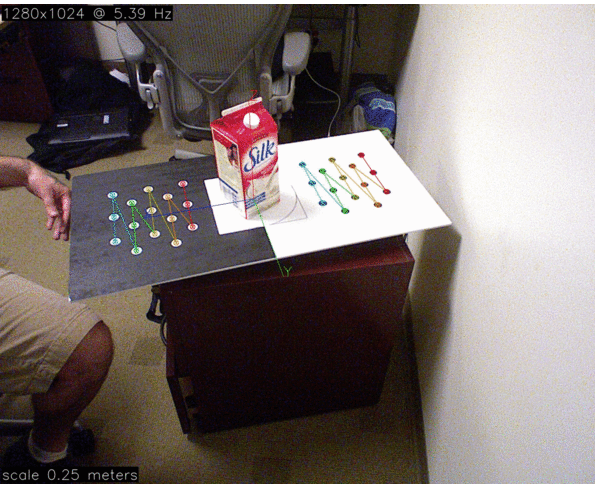
\includegraphics[width=0.5\linewidth]{images/spintable}
\caption{Detection of training pattern for 3D reconstruction of a template from several views. Image taken from \cite{bib:ORK}}
\label{fig:calibpat}
\end{center}
\end{figure}
After templates are trained the detection function can be used with the templates in the database to perform object detection. A drawback of this algorithm is that it does not work with partial occlusions of the object. 
\item \textbf{Tabletop} This algorithm assumes that the objects are on top of a plane (eg. table) that is the biggest plane in the scene. First it finds the planes of the scene identifying which is the one to be considered as table plane, then it segments the objects on top of this plane. After segmentation, the clusters are compared for possible candidates in the database. Finally a iterative process tries to match the object with the candidates and determine which is the best match. A big drawback of this algorithm is that it assumes the objects are rotationally symmetric with no 3D rotation. 
\item\textbf{Texture Object Detector (TOD)} It implements bag of features approach, in which the RGB images from different views of the object are analysed to extract features and build descriptors. The depth information is stored for each view. Then detection stage of the algorithm is performed comparing extracted features with the ones in the database. The drawback in the actual implementation of the algorithm in ORK is that  the pose of detected object can only be obtained in 2D in the RGB image, this due to the fact that only the depth information is taken as another feature in the descriptor and not the whole 3D pose of the object. 
\item\textbf{Transparent Objects} Algorithm focused on detecting transparent objects, there is not much documentation about. A drawback is that the training of the object should be done with a painted version of the object. 
\end{itemize}
After  a month analysing the off-the-Shelf algorithms provided by ORK as well the documentation on how to develop the project in this pipeline, it was concluded that for the project goals ORK was not the ideal solution because of the followings reasons:
\begin{itemize}
\item The algorithms that probably comply more with the needs of the project are Line-mod and Tabletop, since TOD is more focused on analysing 2D data in textured object and not all the objects in a common offices scene have texture.
\item Tabletop will only detect objects with no 3D rotation in the scene, which  in a common office scene is almost impossible to happen since objects can be asymmetric.
\item Line Mode algorithm is a template based matching algorithm, when discussed with the supervisor, it was concluded that the developed solution should be robust against scale changes. In a template based matching recognition approach like this, the scale invariance is difficult to implement and the off-the-shelf algorithm does not have it implement with a lot of robustness. Also the fact that it does not work correctly with partial occlusions represent a big drawback for the project, since one of the goals is to detect the objects even though they are occluded with a partial view of it. Even if this algorithm is used to train each structuring element of the classes (eg. train the leg of the chair), still the developed solution should be robust to some occlusions. This condition is not provided by line-mod and for this reason it was discarded in this stage of the project. 
\item ORK's documentation is very poor since it is in a beta stage, the team struggled a lot with trying to understand the code that has few documentation and comments, as well to use the already off-the-shelf algorithms. The creation of new cells and implementation of other algorithms didn't seem to be a smooth task.  
\end{itemize} 
After doing some research in which other frameworks were available and preferably already implemented or connected with ROS, it was  determined that the Point Cloud Library (PCL) \cite{bib:pcl} is a suitable framework to develop the common office recognition project.
The PCL is an open project which provides built-in functions for pre-processing, registering and analysing point clouds. The documentation is extensive and some companies like Toyota, willow garage and Bosch, as well several universities are contributing to this open project. Regarding the integration of PCL in ROS, there are already available functions to connect PCL with ROS as well some built in functions in ROS that use PCL, which is an advantage for the goals of the project. \\

Literature review was performed at this stage on  how to solve the recognition problem, and it was found that a solution can be to fit geometric primitives like cylinders, spheres and boxes using the point clouds. This gives the advantages in the OOR (Office Object Recognition) project, in the sense that the structural elements of the objects can be described with geometric primitives. For example a chair can be described of 4 cylinders or 4 boxes interconnected, or nearby, to a perpendicular box ( representing the seat of the chair) , and another box can represent the  back support of the chair. With this approach the scale invariant problem can be solved since the descriptors of a class contain relationships between the geometric primitives and not a fixed template. \\

A good example of object description using primitive shapes is \cite{pap2} however this solution is designed basing on database of CAD produced objects which is less difficult than dealing with noisy data of a point cloud. Even though the results obtained are relatively good, the computational time precludes using it for real time applications. In \cite{pap1} presented solution fits very well requirements of this project. The approach involves using RANSAC for primitives fitting and probabilistic graph algorithm approach for recognizing the object. Nevertheless the computational time obtained is quite high due to lack of preprocessing for the point cloud and trying to fit basic shapes on raw obtained data from kinect. The approach that will be proposed in this report,  is trying to decrease computation time by quick preprocessing of the point cloud which allows to run RANSAC in shorter time. In addition we use a simplified graph algorithm without probabilistic approach. Due to the advantages that PCL offers, it was discussed and approved by the project supervisor, to modify the requirements of the project in order to change the vision framework from ORK to PCL. 

\section{Project Management}
\label{sec:planning}
The initial planning of the project, contemplated  the gant diagram setting the milestones shown in figure \ref{fig:plan1}; in which the first two weeks were intended to determine if the ORK framework could provide the necessary software tools and algorithms to develop the application.
\begin{figure}[H]
\begin{center}
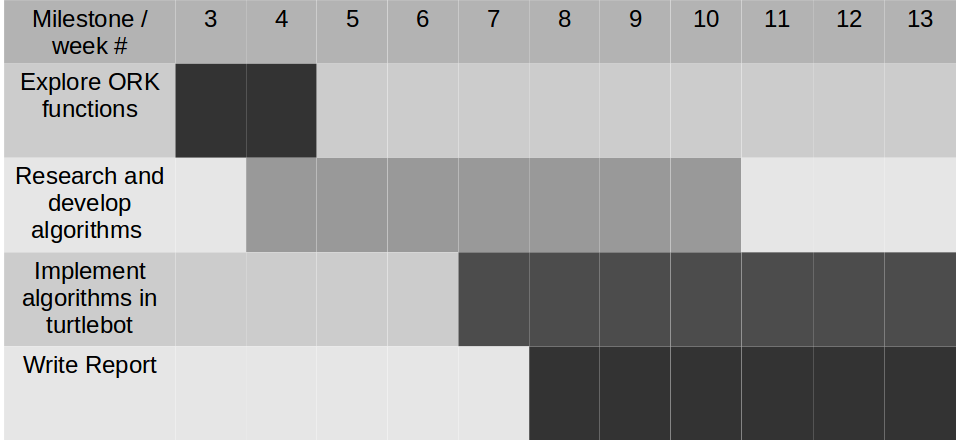
\includegraphics[width=0.8\linewidth]{images/plan1}
\caption{Lobos Solitarios first project planning}
\label{fig:plan1}
\end{center}
\end{figure}

However after analysing the proposed initial tools for developing the project, and determining that ORK was not suitable for the project as described in section \ref{sec:toolseval}, some changes to the project planning were made. The new requirement of 3D mapping added to the project was taken into account and the new time table of the project is shown in \ref{fig:plan2}.
\begin{figure}[H]
\begin{center}
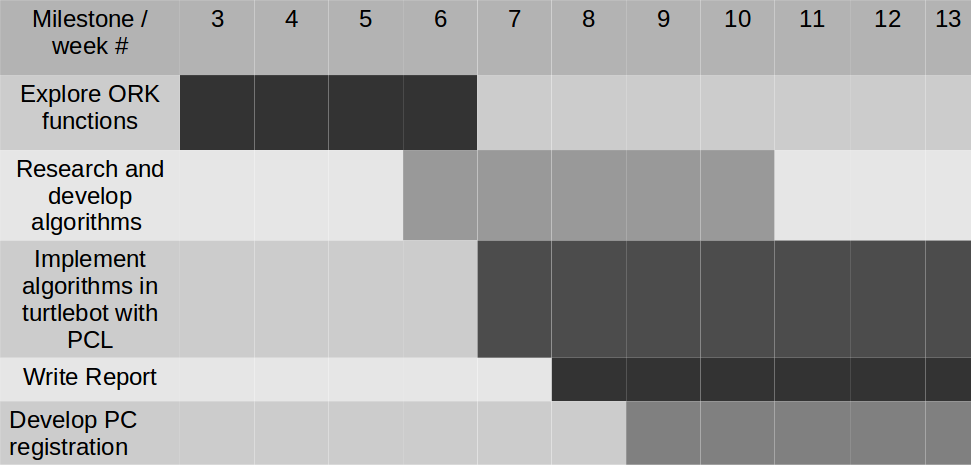
\includegraphics[width=0.7\linewidth]{images/plan2}
\caption{Time table using PCL framework}
\label{fig:plan2}
\end{center}
\end{figure}

It was decided that the work-flow to follow to implement a starting point would be:
\begin{itemize}
\item \textbf{Point Cloud registration}
\item\textbf{Plane Extraction}
\item \textbf{Cluster extraction}
\item \textbf{Geometric primitive fitting}
\item \textbf{Recognition}
\end{itemize}
After having settled down the new goals, and having the advantage modularity provided by ROS for developing, the workload was divided between the members of the team in : Point cloud registration, plane extraction,  clustering and detection.  
The architecture of the developed project is summarized in figure \ref{fig:flowchart}
  \begin{figure}[H]
\begin{center}
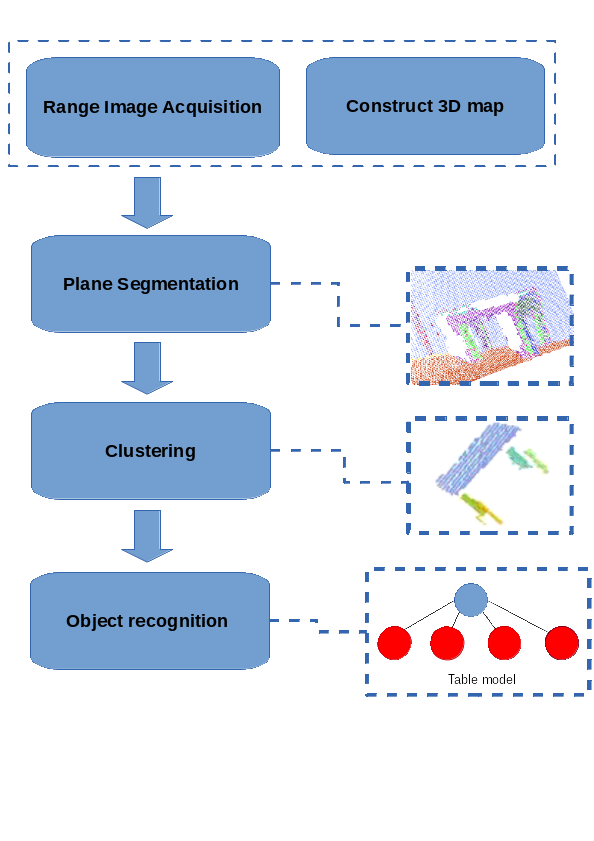
\includegraphics[width=0.7\linewidth]{images/flow_chart}
\caption{Flow chart of lobos solitarios solution architecture}
\label{fig:flowchart}
\end{center}
\end{figure}

\section{3D mapping}
\label{sec:map}
As explained in section \ref{sec:probdesc}, and the new requirement of the supervisor to perform the 3D mapping in this stage of the project; the robot should be able to build a 3D map of the places it has visited, for later use to detect the objects and identify their position in the map as well to merge different views of the object to have a better recognition. The following possible solutions to register point clouds or build the 3D map with the readings of the robot were analysed:
\begin{itemize}
\item CCNY visual odometry and 3D map building
\item PCL point cloud registration
\item Octomap 3D mapping
\end{itemize}

\subsection{CCNY visual odometry}
This package available for ROS can be obtained in \cite{bib:visualodo}, which is a set of tools to  perform visual odometry and 3D mapping. It extracts keypoints from the RGB images and  estimates the motion of a moving RGBD camera. The drawback is that  it does not output a map, and does not perform online SLAM. Offline graph-based SLAM  can be performed to output the 3D RGB map. This approach was not selected for the project since the map is built offline. Also when doing some test, registrations from different views after building the map offline, appeared to have some miss alignments, and the algorithm does not provide a built in function to correct this miss alignments. Other aspect to take into account is that the odometry of the robot is not used in the off-the-shelf approach. Since odometry and localization techniques can be  available in the turtlebot, the use of visual odometry will not take advantage of this. 

\subsection{Point cloud registration using PCL}
PCL has some examples on the usage of the built-in function to iteratively align two point clouds by using the Iterative Closest Point algorithm. This function is useful when the two point clouds are near each other in terms of difference between the scenes, this can be the case of the robot if you take consecutive frames, like for example when moving the turtlebot slowly and registering successive point clouds. This is a starting point but still other problems have to be solved, like how to build the map with the points clouds, which implies position and heading tracking of the robot after localization, to incrementally build the map by registering several contiguous point clouds. 

\subsection{Octomap 3D mapping}
The octomap is a  probabilistic 3D mapping technique which is based in octrees and is described in \cite{bib:octomap}. An octree is a tree type data structure in which each node in an octree represents the space contained in a cubic volume, usually called a voxel. As its name indicates each voxel is recursively subdivided into eight sub-voxels or nodes until a given minimum voxel size is reached. This structure can be observed in figure \ref{fig:octree}, in which the black cube represents the minimum voxels size or depth reached in the tree. 
\begin{figure}[H]
\begin{center}
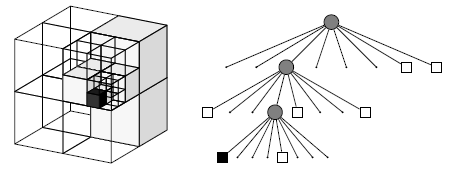
\includegraphics[width=0.8\linewidth]{images/octree}
\caption{On the left the graphical representation of the subdivided voxel. Osn the right the tree representation and position of the voxels. Image taken from \cite{bib:octomap}}
\label{fig:octree}
\end{center}
\end{figure}
In the implementation of octomap the  default depth of the tree is 16 levels, but can be configured to less to speed up the process, with the drawback of having less resolution. Also the convenience of having a hierarchical tree structure, allows to fetch the tree in any level or depth to access different degrees of resolutions as illustrated in  \ref{fig:difrefocto}. 
\begin{figure}[H]
\begin{center}
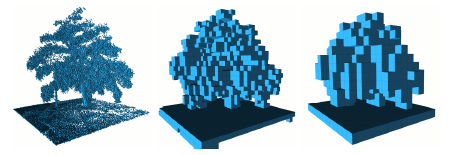
\includegraphics[width=0.8\linewidth]{images/treedifres}
\caption{Different resolutions of the octomap reached when accessing different depth of the tree. Image taken from \cite{bib:octomap}}
\label{fig:difrefocto}
\end{center}
\end{figure}
Using the octree structure as baseline, the octomap implementation stores information in each node about its occupancy state, particularly if the node is free or occupied. Free nodes are created in the area between the  source (3D sensor) and the measured end point along a the ray that joins these two points. Areas that are not initialized implicitly are considered as unknown space. This mixed representation of free, occupied and unknown voxels is useful when building a 3D map in the sense  that the system or robot will know which parts of the map had not been explored yet. For the future goals of the project, this characteristic can be helpful when the robot determines that it needs to move and observe an unknown part of an object that was partially observed before.  In figure \ref{fig:octreefree} is shown an example of the representation of free and occupied voxels in a scene. 
\begin{figure}[H]
\begin{center}
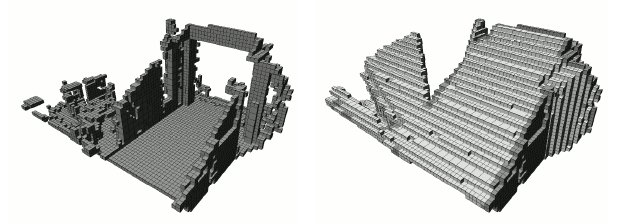
\includegraphics[width=0.8\linewidth]{images/octofree}
\caption{On the left, the representation of occupied voxels. On right the representation of free and occupied voxels. Image taken from \cite{bib:octomap}}
\label{fig:octreefree}
\end{center}
\end{figure}
Another characteristic of octomap implementation is that voxels can be pruned to reduce the amount of data to store, for example if all the children of a node are free, they can be gathered into a free big voxel. \\
Octomap provides robustness to sensor noise and the environmental changes by implementing a probabilistic approach to determine the current occupancy state of each node. Specifically it computes the actual free or occupied probability with an occupancy grid method that needs the current measurement, a prior probability (a previous state) and a previous estimate. The node is considered free or occupied when it reaches a certain threshold in its occupancy probability value, in this way the noise is diminished. For example, if after \textit{n} readings a voxel was labelled as occupied,  \textit{n} more readings are needed to change its state and label it as free, this when considering that free and occupied probabilities  have the same weight. Having this methodology apart from giving robustness to noise, it allows the map to readjust in some cases to changes in the environment and  misalignments provoked by a failure in the localization method of the robot. This property is very convenient for the project, to compensate a little bit the lack of accuracy in turlebot's odometry and localization built in algorithms.
After analysing the theoretical advantages of using octomap, it was decided to propose it as 3D mapping solution for the office object recognition. 
Octomap package does not perform localization, it needs a 2D map and a transformation matrix of the sensor to perform the 3D mapping. For this reason another node has to perform the localization and 2D maping. To provide an starting point to this problem, the already implemented 2D Slam provided in ROS was used to build a 2D map with the ease of use of gmapping node present in turtlebot\_ navigation package. This node emulates a range laser scanner with range image of the kinect sensor to input it as observations to the SLAM algorithm. The output map and the sensor transform of gmapping are fed to the octomap to give the information on which part of the 3D map it should assign the occupancy probabilities. A block diagram of the connections between the mapping elements is shown in figure \ref{fig:OctowithROS}.\\

\begin{figure}[H]
\begin{center}
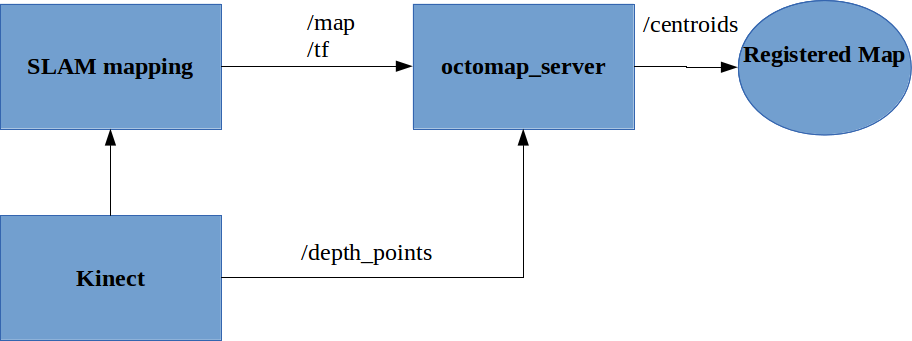
\includegraphics[width=0.8\linewidth]{images/diagocto}
\caption{Octomap integation with ROS in the project}
\label{fig:OctowithROS}
\end{center}
\end{figure}
Some parameters to configure in the octomap node are:
\begin{itemize}
\item \textbf{resolution}.- This parameter is expressed in meters and sets the resolution of the map in terms of minimum voxel size. With more resolution the construction  of the map will be slower having more dense point clouds, but having more precision.   
\item \textbf{sensor model hit and miss probabilities}.- Each endpoint or 3D measurement increases the probability that a voxel is occupied by \textit{hit} value, each other voxel's probability along the ray to the endpoint is decreased by the \textit{miss} value. Increasing the hit probability and decreasing the miss probability at the same time, makes the algorithm trust the sensor more after one measurement, since a hit has more weight than the free space (miss).
\item \textbf{sensor model max and min probabilities}.- This values define the lower and upper bound when changing the state of a voxel into free or occupied label. If min is increased and  max decreased at the same time, will enable fast updates at the cost of more sensor noise appearing in the map.
\item \textbf{filter ground}.- This is a boolean variable that when set to true performs a ground plane subtraction algorithm. 
\item \textbf{latch}.- This boolean variable is focused more for visualization purposes, when true, all the topics are created in each map update. When building the map, is better to set this value to false. 
\end{itemize}

An example of a 3D map of a real scene  recorded by the turtlebot is shown in figure \ref{fig:octoscene}, where the 3D map point cloud of the centroids from the voxels is accessed and displayed. This was the result of circumnavigating the turtlebot through Leonard Horner Lounge. As it can be seen, the ground plane is subtracted and different views are merged. 
\begin{figure}[H]
\begin{center}
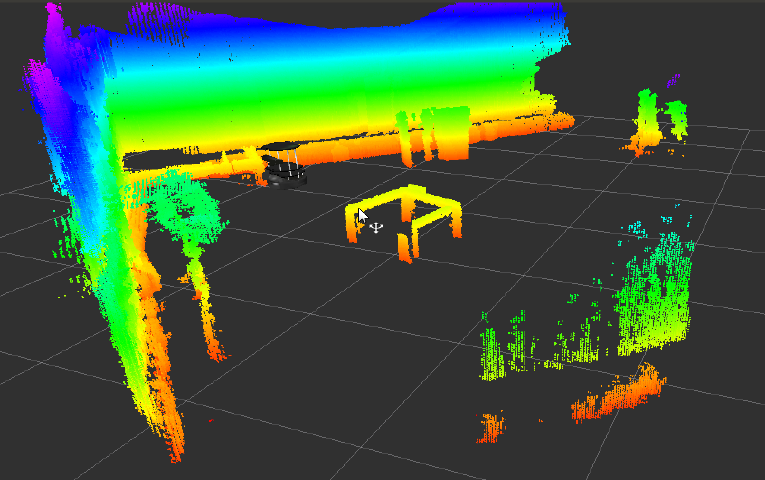
\includegraphics[width=0.6\linewidth]{images/figoctomap}
\caption{Octomap 3D mapping of a scene with ground plane substraction and a resolution of 0.025 meters was configured for the minimum voxel size }
\label{fig:octoscene}
\end{center}
\end{figure}

Octomap gives a suitable starting point for 3D mapping, however after doing some tests the 3D mapping was not always accurate probably due to the cumulative error in the localization after several time of circumnavigation. Even-though the map re-adapts to changes in the environment due to its probabilistic approach, sometimes the  errors in localization provoked by a inaccurate SLAM mapping, produces that the walls or objects appear to have shadows or ghosts. It has to be taken into account that to change the label of a voxel it has to be in the line of sight of the sensor. For example when having a voxel labelled as wall, and after circumnavigating \textit{x} time and observing again  the same place but with a bad localization, can happen that now the wall appears to be closer. New voxels will be added since the system thinks that free space is now occupied. Since the previous wall now is not reachable due to localization misalignment, it will never be updated to be a free voxel. This can be fixed by improving the localization module, probably by adding a more accurate range sensor, like a laser range sensor. 

\section{Plane Segmentation}
\label{sec:plane_segmentation} 

To make the search of primitives easier we first decided to segment the data following some rule that would split it into smaller sets but at the same time would not split the objects. After doing some literature review we found a paper \cite{bib:planes_paper} were they propose a method to detect and segment planes in a fast way. In their case, as in ours, the 3D data information comes from RGB-D images were the range data is used to project the pixels into 3D positions. They use an innovative approach where the neighbouring in the 3D space is approximated with the pixel neighbouring in the image. This algorithm is said to be able to run at 7 frames per second, ideally its output should be an initial approximated clustering that could be polished on later steps.\\

Finally they propose some methods to do a fast approximation of the clustering of the planes.\\

\begin{figure}[!htbp]
  \begin{center}
    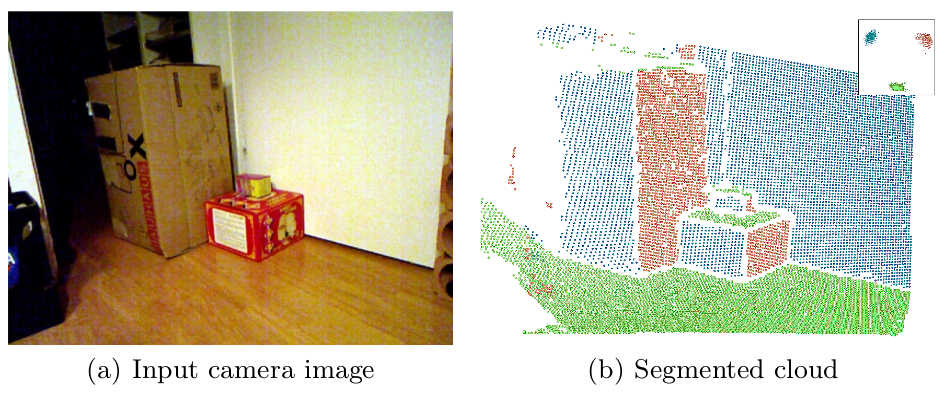
\includegraphics[width=8cm]{./images/segmentation_result.png}
    \caption{Example segmentation. Image from \cite{bib:planes_paper}}
    \label{fig:example_segmentation}
  \end{center}
\end{figure}

\subsection{Algorithm}
\label{sub:plane_algorithm}

The algorithm consists of 3 main parts:

\begin{itemize}
  \item Normals computation
  \item Normals clustering
  \item Parallel planes distinction
\end{itemize}




\subsubsection{Normals Computations}

One way to represent planes is by its normal and one point belonging to the plane. To determine if two points belong to the same plane a first step is to compute the Normal vector in each of the two points, then if they have a similar normal it could give an initial estimation of the points belonging to the same plane.  To compute the normal of one point the information of its neighbours is needed and so  the first problems arises, how can we find the neighbour of a point? One approach is to use the closest points using KNN with some fast implementation. Once this points are found a plane can be fit and from it calculate its normal.\\

The problem of this approach is that the search of neighbours can be very computationally expensive even when using fast algorithm that only approximate the result. Also, if many points are fit to the plane, the computation of the normal vector using eigen decomposition can also be computationally expensive. \\

In the proposed method both steps are substituted by much simpler and faster operations.\\

First of all the algorithm assumes that two pixels in the range image will still be neighbours once they are projected in the 3D space. This will not hold on the edges of planes but in general it can be accepted. At this step the algorithm computes two tangential vectors of the point using the difference between the neighbours. One of the vectors is extracted form the difference between the projected above pixel and the projected below pixel, the other vector is computed in the same with the left and right neighbour pixels. In Figure~\ref{fig:example_segmentation} it can be seen which are the neighbours of one pixel and how the normal is consistent with this neighbouring. This two vectors are considered tangential to the plane which the current point belongs to. Then the cross product of this two tangential vectors is used to obtain the normal vector of the plane of the current point.\\

\begin{figure}[!htbp]
  \begin{center}
      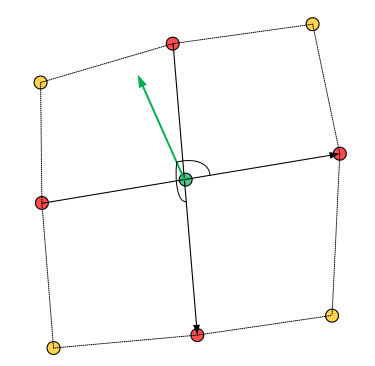
\includegraphics[width=8cm]{./images/normal_example.png}
      \caption{In red the four neighbours of the current pixel. In green the current pixel and its normal. Image from \cite{bib:planes_paper}}
    \label{fig:example_segmentation}
  \end{center}
\end{figure}

\subsubsection{Normals Clustering}

After normals are computed for each of the points, a second step comes in which clustering of similar normals is carried on with the idea that similar normals will belong to the same plane. To do the clustering different iterative algorithm like k-means could be used but to avoid computational cost a different method is used. In this case an octree is build with the normals as positions, this way similar normals will fall in the same octree leaf. Initially points with normals falling in the same octree leaf will be considered part of the same plane.\\

The performance of this method is very sensitive to the resolution of the octree. Too large resolution will not be able to distinguish between similar planes and too small resolution will oversegment the planes. This problems are partially attenuated with two methods. This first one is to smooth the normals using again the range image neighbourhood idea. Every component of the tangential vectors ($XYZ$) is set up with the shape of an image and a Gaussian filter is applied to it. This makes the normals more homogeneous removing small changes.\\

A second method is to compare the clustered planes by their mean and to merge them if we decide that they are very similar. This also solves the problem of one plane cluster falling between two final leafs. This problem can be seen in Frame~\ref{fig:premergin} where the normals of the background wall have been clustered into two different planes (yellow  and green). The result of solving this problem can be seen in Figure~\ref{fig:posmerging} where the background is now one solid cluster.\\ 


\begin{figure}[!htbp]
  \begin{center}
    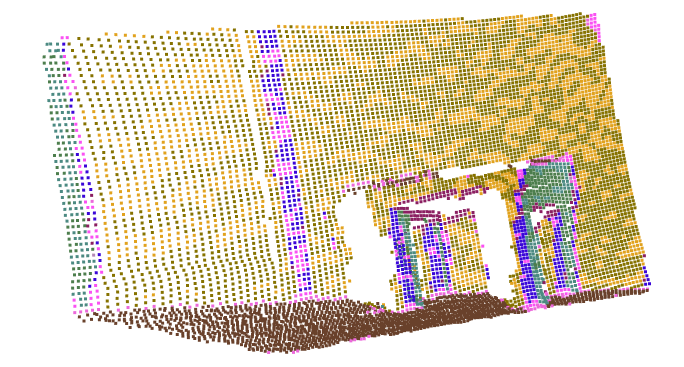
\includegraphics[width=8cm]{./images/premergingSegmentation.png}
    \caption{Plane segmentation with background points falling into two different clusters.}
    \label{fig:premergin}
  \end{center}
\end{figure}

\begin{figure}[!htbp]
  \begin{center}
    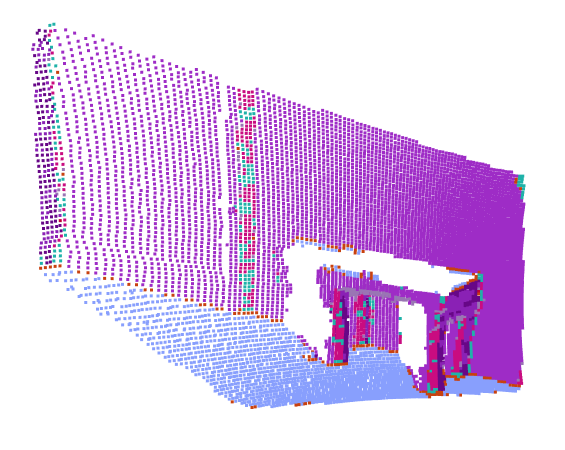
\includegraphics[width=8cm]{./images/midSegmentation.png}
    \caption{Clustering correction with mean computation and merging.}
    \label{fig:posmerging}
  \end{center}
\end{figure}

\subsubsection{Parallel planes distinction}

So far the algorithm is  able to distinguish between planes with different normals but parallel plans share a normal while not being the same plane. During this third step this differentiation is carried out.\\


The feature used to distinguish between points of different parallel planes is the distance between the point and the plane defined by the mean normal of the cluster and a set point, usually the origin (0,0,0). Points from the same plane will have the same distance to this reference plane.\\

Finally to cluster this distances the same technique from the previous step is used. An octree is feed with the distances as position positions. Distances falling in the same final leaf are considered to be part of the same plane. In Figure~\ref{fig:final_segmentation} there is the final result of the plane segmentation after this step is applied, it can be seen that in contrast with~\ref{fig:posmerging} the background plane and the frontal part of the table are now not part of the same plane.\\

\begin{figure}[!htbp]
  \begin{center}
    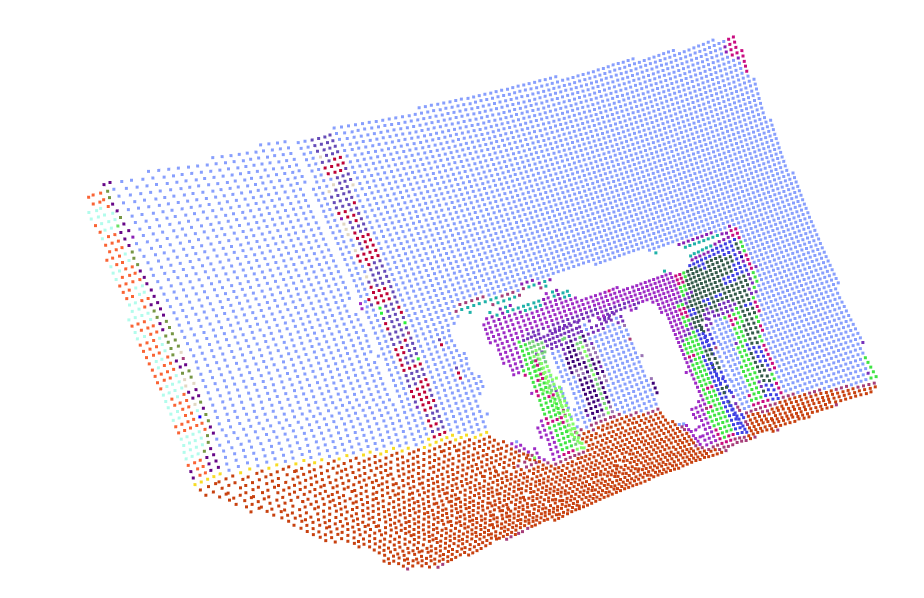
\includegraphics[width=8cm]{./images/finalSegmentation.png}
    \caption{Final segmentation after similar cluster merging and parallel planes differentiation.}
    \label{fig:final_segmentation}
  \end{center}
\end{figure}


\subsection{Algorithm implementation with PCL}
\label{sub:algorithm_implementation_with_pcl}

The described algorithm in section~\ref{sec:plane_segmentation} has been implemented using PCL~\cite{bib:pcl}. Three main objects from the library have been used: \textit{PointCloud}, \textit{RangeImage} and \textit{Octree}.\\

\begin{itemize}
    \item \textbf{PointCloud}: class that contains a set of points representing a point cloud. We use this class to contain the clustered point clouds. This class can be used to iterate through points and can be easily displayed. It is a template class and can be instantiated with different types of points (plane points, points with color, point with normal\ldots).
    \item \textbf{Octree}: implementation of an octree. After assigning data to it, it is possible to iterate through the final leafs and accessing the list of points of each  one. This was one of the problematic points during the implementation because the interface had been updated and all the on-line examples used one class method that did not exist any more. We had to look at the actual code of the class to find out how to iterate through the leafs which is not trivial on a library of this size and complexity. During the clustering the position was given by the computed normal but somehow the actual point should also be there in order to recover it after the clustering. We used the Octree class with points with normals where the point was the normal and the normal was the point.
    \item \textbf{RangeImage}/\textbf{PlanarRangeImage}: this class represent an image where each pixel has four fields: the actual range data, and the $XYZ$ position of the pixel projected in the 3D space. This is exactly  the type of information needed by this algorithm. During the implementation the range image was computed from a point cloud read from disk. Afterwards the range image was obtained from a ROS message. The difference between RangeImage and PlanarRangeImage is that the PlanarRangeImage is created from range data that has been previously rectified using the calibration of the camera, this is the type of data that is published in ROS.
\end{itemize}

The first step of the algorithm as explained is to subtract neighbour points in order to calculate the tangential vectors, we use this step to copy the range image data into openCV data types that will be used later on. The next code is applied to every point fo the image in order to obtain the horizontal tangential vector, something similar is done for the vertical case:\\

\begin{lstlisting}
// horizontal vector calculation
hori->at<cv::Vec3f>(j,i)[0] = 
range_image_ptr->getPoint(i-1,j).x - range_image_ptr->getPoint(i+1,j).x;
hori->at<cv::Vec3f>(j,i)[1] = 
range_image_ptr->getPoint(i-1,j).y - range_image_ptr->getPoint(i+1,j).y;
hori->at<cv::Vec3f>(j,i)[2] =
range_image_ptr->getPoint(i-1,j).z - range_image_ptr->getPoint(i+1,j).z;
\end{lstlisting}
% subsection algorithm_implementation_with_pcl (end)

The advantage of having now the data in openCV format is that we can now apply the Gaussian filters that we mentioned. Also the vectors can be accessed on by one as if they were RGB data. This way the computation of the cross product straight forward.

\begin{lstlisting}
// Gaussian filtering on the tangential vectors
cv::GaussianBlur(*hori, *hori, cv::Size(3,3), 0);
cv::GaussianBlur(*vert, *vert, cv::Size(3,3), 0);
.
.
.
// Cross product of the vertical and horizontal tangential vector
crossVector = hori->at<cv::Vec3f>(j,i).cross(vert->at<cv::Vec3f>(j,i));
\end{lstlisting}

After this step we create a pcl point cloud with points with normals which will be used to feed the octree. We need to use the norm of the point as the position and we will use the left space to encode the original point. This way the point can be easily retrieved after the clustering. Next there is an example of the creation of such points.

\begin{lstlisting}
pcl::PointXYZINormal p;
cv::Vec3f n = normals->at<cv::Vec3f>(j,i);

p.x = n[0];
p.y = n[1];
p.z = n[2];
p.normal_x = range_image_ptr->getPoint(i, j).x;
p.normal_y = range_image_ptr->getPoint(i, j).y;
p.normal_z = range_image_ptr->getPoint(i, j).z;
\end{lstlisting}

Once the normal point cloud has been created we feed an octree with this data and we iterate over all the final leafs that have data. With the points from every final leaf a new point cloud is created. All this point clouds are then returned in a std::vector. An extra step is done after the clustering where all cluster are comared to each other using its mean value and merged if they are similar enough.\\

\begin{lstlisting}
pcl::octree::OctreePointCloud <T> normals_ot (); 
normals_ot.setInputCloud(pc_ptr);
normals_ot.addPointsFromInputCloud();

my_OctreeIterator itL (&normals_ot);
//Iterate through all the leaf nodes of the octree
while (*itL ) {
    vector<int> idxList;
    my_LeafNode *node =  (my_LeafNode*) itL.getCurrentOctreeNode();
    
    node->getContainerPtr()->getPointIndices(idxList);

    pcl::PointCloud<T> cluster;
    for (size_t i = 0; i < idxList.size();  ++i) { //idxList.size();
        int idx = idxList[i];
        T p = (*pc_ptr)[idx];
        
        cluster.push_back(p);	
    }
    clusters.push_back(cluster);
    itL++;
}
\end{lstlisting}

Finally from each clustered point cloud a new point cloud is created in order to differentiate between parallel planes (which have the same norm). This new point cloud will have the distance from the point to the reference plane. The same clustering technique with an octree is applied to this point cloud. A new point from this point cloud is created as follows:

\begin{lstlisting}
normal.x = meanNorm[0];
normal.y = meanNorm[1];
normal.z = meanNorm[2];
point.x = normal_clusterList[i][j].normal_x;
point.y = normal_clusterList[i][j].normal_y;
point.z = normal_clusterList[i][j].normal_z;

// Encode position as distance from point to plane
p.x = distPointToPlane(point, normal);
p.y = 0;
p.z = 0;
p.normal_x = normal_clusterList[i][j].normal_x;
p.normal_y = normal_clusterList[i][j].normal_y;
p.normal_z = normal_clusterList[i][j].normal_z;
\end{lstlisting}

\subsection{Implementation Problems}
\label{sub:implementation_problems}

The main difficulty we had during the implementation of this paper was to find documentation from the methods of the octree class. More concretely how to iterate through the leafs. Initially all the found references mentioned a method \textit{getData()} that did not exist in our case. Eventually we were able to find the new way of iterating the octree.\\

During the implementation of the algorithm we used a point cloud from disk which its points were then projected to an image plane.  Apparently this process caused a resampling from the data going from the order of hundreds of thousands to the order of thousands. This algorithm could not be tested with real data until integrated with ROS. At this point the algorithm was not only much more slower (caused by the large amount of data) but also the segmentation was not working correctly in many cases (as was seen during the demo) that had been working previously. This problem could come first from a problem with the implementation or second from an unexpected change of type of data between others. It is possible that the type of data given by the Kinect is somehow different to the data obtained with the projection used during the implementation. \\

% subsection implementation_problems (end)


\section{Object Recognition module}
\label{sec:recognition}

This section discusses algorithm used for the object recognition in \emph{lobos\_prmtv\_process} node after planes segmentation was performed. In the following subsections each step is described in detail pointing out the problems and alternative approaches taken into consideration. The general pipeline followed by this module is presented on figure \ref{fig:pipeline}. However due to poor results obtained in some sections the final approach deviated slightly from the initial idea.


\begin{figure}
\begin{center}
  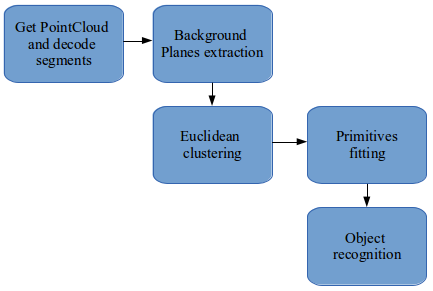
\includegraphics[scale=0.7]{images/pipeline}
  \caption{Object recognition pipeline after plane segmentation.}
  \label{fig:pipeline}
  \end{center}
\end{figure}
\subsection{Planes decoding}
The node subscribes to topic \emph{planes\_segmented} which publishes cloud with various colors for the planes extracted. First in order to be able to work with obtained plane segments they have to be decoded. For that purpose we use a map where RGB values are considered as a key while the map value points the index of cloud in output vector. General algorithm of the function \emph{getColorSegment()} is shown on figure \ref{code:algo}.

\begin{figure}[H]
\begin{center}
\begin{lstlisting}
for each point i in point cloud
  if in map exists key 'i.RGB'
    add i to point cloud in output vector,
    with idx == value of map for this key
  else
    create new map entry with value
    create new point cloud in output vector
    add i to created point cloud
\end{lstlisting}
\caption{Pseudo-algorithm for decoding the segments from the color cloud.}
\label{code:algo}
\end{center}
\end{figure}

The disadvantage of this solution is that we have to decode already segmented in other node point cloud. Modularity comes at the cost of additional computation. This simple solution was used due to the lack of appropriate message that could handle e.g. vector of point clouds. The most optimal solution would be to create ROS message able to do so. Having that, one could avoid decoding the segments, because they would be passed directly from the segmentation node.

\subsection{Plane extraction}
Objects are most commonly local areas in the point cloud scene. Therefore in order to focus just on the relevant part of the data, we extract unnecessary planes obtained in segmentation. The first problem when performing this task is how to determine which planes are irrelevant for particular algorithm. It can be safely assumed that walls are least relevant segments, as well as ground floor, which however might be usefull e.g. to determine the basis of objects, calculate their height etc.
\newline
\indent Having the vector of segments we can either set a threshold for number of points in segment or remove the biggest segments assuming that floor and wall will usually cover the biggest parts of the scene. Both methods are strongly scene dependent and prone to errors in various scenes cases. We applied size threshold empirically determining the value. Using the wooden blocks, on which most of the test was performed, we applied thresholding at different levels. As a result we found that 1/10 of the total scene point cloud size is a	 threshold sufficient to maintain important parts.
\newline
\indent Obviously this is a very trivial approach tested in simple scene cases where object can be clearly distinguished. This solution would fail in case where the environment is cluttered with multiple planes or the object ocupies most of the registered cloud points. A better approach would involve determining which segment is the floor plane first and then finding planes vertical to this plane. It can be achieved using the sensor position which can be obtained in PCL. 

\subsection{Euclidean clustering}
\indent It can be observed from segmentation results that primitive parts like table legs are actually composed of few segments. Since the aim is to be able to recognize basic shapes represented by primitives these subsegments of the primitives have to be merged into one cluster. This can be achieved by euclidean clustering.
\newline
\indent In order to cluster the segments,the algorithm for given distance threshold finds the nearest neighbour for a particular point and if it meets the requirements it proceeds to this point and repeats the procedure until there is no more points that can be assigned to the cluster. Since computational time is crucial, the PCL euclidean clustering uses KdTree which allows to tremendously decrease this parameter. 
Again the parameters problem arises in this case. Crucial input in case of euclidan clustering is the minimum/maximum possible size of the cluster and threshold distance between points. This will obviously vary for different input data. Size constraints for the clusters were determined again experimentally like in case of plane extraction described in previous section. Determining the distance threshold is more problematic since it will strongly depend on range at which the object was registered. Therefore the appropriate solution would be to choose this coefficient basing on the range information, however we followed the less robust solution of just setting it to constant value. This significantly limits robustness of the overall algorithm because it will perform well only for objects registered at certain range of distances from the sensor. 
\subsection{Primitive fitting}
Recognizing primitive shapes in the clusters gives the possibility to describe a bigger (in terms of type variation) set of objects hence one is able to better process obtained data. For this purpose RANSAC algorithm was used as in \cite{pap1}. It allows to iteratively estimate a mathematical model, from a given input data. Since the considered problem requires generic detection, this solution fits perfectly. Algorithm is already provided with many basic shape models in PCL and in addition for clusters on which the tests were performed it did not influence the computational time in a significant way.
\newline
\indent The general idea of RANSAC is quite simple. Having the mathematical model it iterates through the input data and basing on predetermined threshold values it's trying to fit given point into the model thus separating inliers from outliers. The higher is the number of iterations in RANSAC that is used the better model approximation will be obtained.
\newline
\indent RANSAC however is no different than previously described parts of algorithm in terms of problems. It suffers even more from the parameters that are passed to the algorithm in order to fit the shape. The result depends on about 5 parameters (depending on the application) which are hard to determine in a generic way for every scene. Problem with obtaining good results in terms of primitive shape fitting was the reason to slightly change and simplify the algorithm. Instead of using primitive shape specific descriptions, only their orientation was taken into consideration in order to divide the data into classes of of horizontal (planes) and vertical (supports) objects.  
\begin{figure}
  \begin{center}
    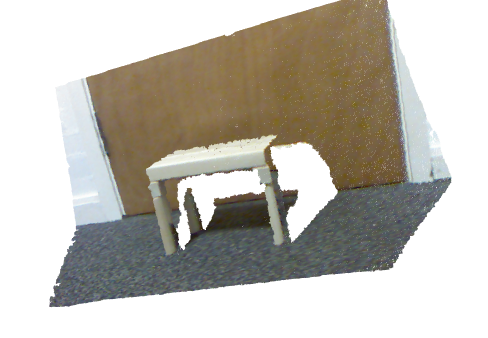
\includegraphics[scale=0.5]{images/rgbTable}
    \caption{Input point cloud.}
    \label{fig:rgbTable}
  \end{center}
\end{figure}

\begin{figure}
\begin{center}
  \begin{tabular}{|c|c|}
  \hline
  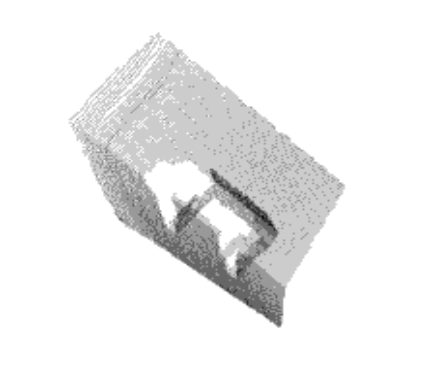
\includegraphics[scale=0.4]{images/cloud1} & 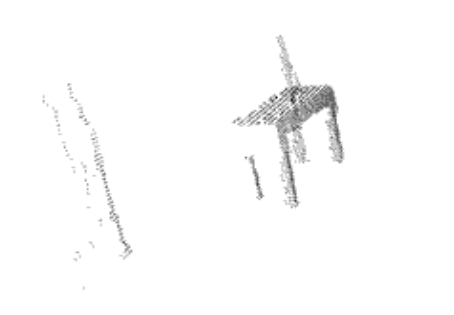
\includegraphics[scale=0.4]{images/cloud2}\\
  \hline
  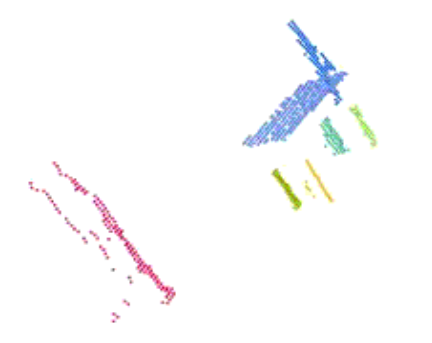
\includegraphics[scale=0.4]{images/cloud3} & 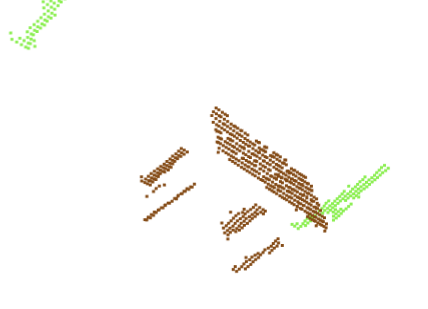
\includegraphics[scale=0.4]{images/cloud4}\\
  \hline
  \end{tabular}
  \caption{Result of the algorithm without using basic shapes fitting. Top row: original input cloud, cloud with extracted planes. Bottom row: euclidean clustering, final result with grouping}
  \label{fig:clustResult}
  \end{center}
\end{figure}
\subsection{Primitives orientation}
Primitives orientation function \emph{getDirection()} was implemented in order to determine whether a particular cluster is oriented verticaly or horizantaly. It was designed for the simplified version of object recognition due to poor results of basic shape fitting explained in previous section.\newline
\indent The function makes use of \emph{pcl::getMinMax3D()} function which for input cloud returns maximum and minimum points with respect to each axis. Taking into consideration known orientation of the sensor, one is able to determine difference between horizontal and vertical(w.r.t. sensor) max/min points of the cloud. The higher difference indicates whether cluster can be considered as vertical or horizontal. This solution is prone to errors in case where cluster has lonely points far away from the main cluster which will change the final result. However in this case this problem is neglected by applying function only after euclidean clustering which makes such a situation impossible. More generic solution for this function could be implemented by using standard deviation of the points from the main axes.

\subsection{Object recognition using graph algorithm}
The final problem of recognizing the object using obtained in the processing pipe clusters is solved with use of graph algorithm presented in \cite{graph}. The object recognition based on primitives can be simplified to finding predefined pattern in a graph where vertices are the primitives and edges are created depending on the euclidean distance between clusters. \newline
\indent The distance is calculated by function \emph{getMinDist()}. Using KdTree created for one cloud, one is able, for given input point, to quickly find the nearest point in the second cloud where the minimum distance will be the minimum distance between two clouds.\newline
\indent As mentioned previously due to poor results of basic shape recognition, the graph was implemented with use of just two types of vertices - horizontal planes and vertical supports. 'Table' object pattern is described as:
\begin{itemize}
  \item 3 vertical supports
  \item 1 horizontal plane
\end{itemize}
Search is computed with recursive algorithm. For every vertex in the graph it is recursively compared to every vertex in the object pattern graph. 
Then it compares every neighbour vertex to vertex neighbour in object pattern graph. The general representation of the graph algorithm is presented on figure \ref{graphAlg}.


\begin{figure}
\begin{center}
  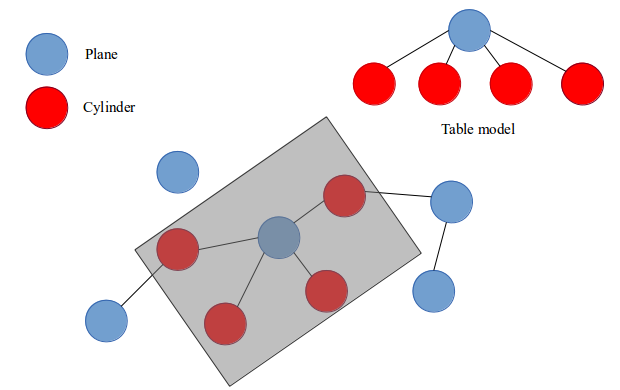
\includegraphics[scale=0.5]{images/graph}
  \caption{Simple graph algorithm visualization for table recognition problem.}
  \label{graphAlg}
  \end{center}
\end{figure}

\section{Results and Evaluation}
Taking into consideration segmentation part of the module for an input cloud presented on figure \ref{fig:rgbTable}, figure \ref{fig:clustResult} presents consequent processing step of the module. Presented cluster grouping was obtained for quite specific parameters adjusted to the particular scene and from different view might not yield such a promising result.
The recognition solution was tested outside of ROS framework, on the set of 27 simple scenes (object in the middle, floor and walls) where 12 of them included table object and 15 did not. It is a small sample however taking into consideration simplicity of the scene it shows that solution does not perform really well. Results shown in figure \ref{fig:resultChart}.

\begin{figure}
\begin{center}
  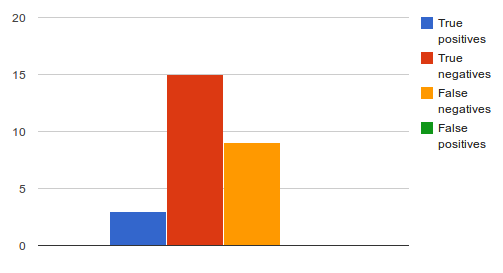
\includegraphics[scale=0.7]{images/resultChart}
  \caption{Results of applying algorithm to set of 27 simple scenes.}
  \label{fig:resultChart}
  \end{center}
\end{figure}

Part of the false negatives results is due lack of enough vertical/horizontal supports visible in the point cloud. Another case is where the segmentation fails which is shown on the figure \ref{fig:fail}.
\begin{figure}
  \begin{center}
    \begin{tabular}{|c|c|c|}
    \hline
      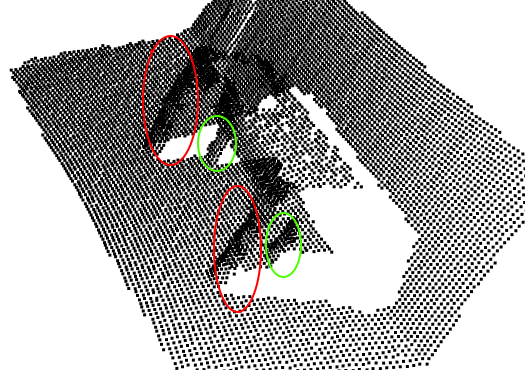
\includegraphics[scale=0.3]{images/fail} & 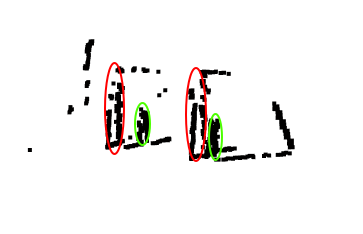
\includegraphics[scale=0.3]{images/failVer} & 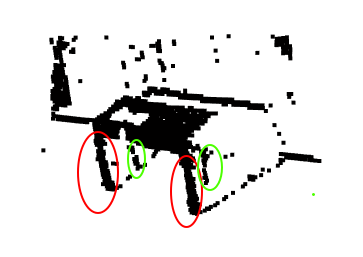
\includegraphics[scale=0.3]{images/failHor} \\
    \hline
    \end{tabular}
    \caption{From left: original image, vertical supports, horizontal segments. Color spheres indicate the same elements on consequent pictures.}
    \label{fig:fail}
  \end{center}
\end{figure}
As it can be seen on this example, front supports and top plane of the table were clustered as one even though in vertical segments we also have parts of table supports. This is result of aforementioned parameters dependent on how the cloud was regiestered as far as sensor position with respect to objects is concerned. Moreover one can notice that supports are clustered in z-direction(perpendicular to sensor plane) which gives not the most elegant solution, since single supports  resembling lines, cylinders or cones are desired. In future work, one should take into consideration removing outliers from the supports taking into consideration that support in z-x (w.r.t. kinect sensor) plane should form a concetrated cloud, perfectly a circle or elipse. 

 Nevertheless taking into consideration favourable conditions of the environment one can conclude that algorithm needs to be improved. However the \textbf{average computational time} registered during this test was \textbf{1.088s} which is better than in \cite{pap1}, where on average it took 19s for object recognition.

\section{Conclusions and Future Work}
\label{sec:Future Work}
An initial approach to the common office recognition problem was developed in this report. The final results of the implemented solution are far from being a robust, at least in the present form. It may serve as a good basis for further work. In this section the main areas that should be improved are pointed out as well things that, if changed, might improve performance.
\begin{itemize}
    \item \textbf{Plane Segmentaiton} the implemented algorithm for plane segmentation had some implementation problems as pentioned in \ref{sub:algorithm_implementation_with_pcl}. The problem that made it not work on the real sensor data should be found and fix. The current version is fast when applied to the data used from the development up 0.7 seconds but it takes about 5 seconds on real data because the amount of processed points is much larger. In \cite{bib:planes_paper} it is claimd that the algorithm should be able to run up to 7 frames per second with the full amount of data so it should be possible to optimize the used code in future implementations. Also further testing should be performed.

\item \textbf{3D mapping} To improve 3D mapping accuracy, a better 2D map construction and localization should be accomplished. If this is not possible, another approach should be developed,  like using PCL point cloud registration and solving the correspondence problem of the registered point cloud position in the 3D map. Due to the actual phase of the project in which the plane segmentation algorithm works with only the range images of the kinect sensor, the  map constructed by octomap algorithm is not yet used in the project. This team settled a starting point in this area, for future work, the integration of the output 3D octo-map containing the centroids of the voxels should be developed. A evaluation to know if  resolution of the 3D map  is suitable to perform a good object recognition when the project is more advanced, should be developed.
  \item \textbf{parameters scaling} - As it was mentioned in first three sections of object recognition part, algorithms will suffer from changes in scale at which the scene is observed and this is the biggest problem of current pipeline especially when using RANSAC. It could be solved with the module which could automaticaly compute particular parameters basing on some predefined rules with respect to distance from the sensor
  \item \textbf{probabilistic graph algorithm} - once the pipeline general performance is improved so that acceptable results are obtained, probabilistic approach as in \cite{pap1} seems to be more prudent solution as long as it does not influence computational time significantly.
\end{itemize}

We implemented a novel approach for primitives-based object recognition, with use of quick preprocessing of the primitives before fitting. The main problem behind making this solution robust is the complexity of all modules combined together. Due to high dependence of each module on determined parameters, the whole system becomes not reliable enough. However we have shown that, in favourable conditions, the pipeline is capable of object recognition by the extraction of oriented sub-clusters from point clouds. Also, our implementation should provide a good starting point for further research into this problem.

\begin{thebibliography}{9}

\bibitem{bib:semantic}
  Jorg Stuckler, Nenad Biresev, and Sven Behnke
  \emph{ Semantic Mapping Using Object-Class
Segmentation of RGB-D Images}.
  In Proc. of the IEEE/RSJ Int. Conf. on Intelligent Robots and Systems (IROS), Vilamoura, Portugal, October 2012.
  
  \bibitem{bib:ORK}
  Willow Garage Inc.(2013), 
  \emph{The Object Recognition Kitchen}. 
  \url{http://wg-perception.github.io/object_recognition_core/}
  
  \bibitem{bib:OCV}
  Itseez.(2013),\emph{Open Source Computer Vision Library}. 
  \url{http://opencv.org/}
  
  \bibitem{bib:ROS}
  ROS foundation.(2013)
  \emph{Robot Operating System}.
  \url{http://www.ros.org/}
  
  \bibitem{bib:ecto}
  Willow Garage, (2011).
  \emph{Ecto}
  \url{http://plasmodic.github.io/ecto/}
  
  \bibitem{bib:visualodo}
  Ivan Dryanovski, Roberto G. Valenti, Jizhong Xiao. \emph{Fast Visual Odometry and Mapping from RGB-D Data}. 2013 International Conference on Robotics and Automation (ICRA2013)
  \url{http://wiki.ros.org/ccny_rgbd}
  
  \bibitem{bib:pclregis}
  PCL org.(2013)
  \emph{How to incrementally register pairs of clouds}
  \url{http://pointclouds.org/documentation/tutorials/pairwise_incremental_registration.php#pairwise-incremental-registration}
  
   \bibitem{bib:octomap}
   Armin Hornung, Kai M. Wurm, Maren Bennewitz, Cyrill Stachniss, Wolfram BurgardOcto.\emph{Map:An Efficient Probabilistic 3D Mapping Framework Based on Octrees}. In: Proc. of the ICRA 2010 workshop on best practice in 3D perception and modeling for mobile manipulation
   
   \bibitem{bib:pcl}
   Radu Bogdan Rusu and Steve Cousins. \emph{3D is here: Point Cloud Library (PCL)}
  .IEEE International Conference on Robotics and Automation (ICRA). 2011. Shanghai, China.
  \url{http://pointclouds.org/}   
  
   \bibitem{bib:linmode}
   Stefan Hinterstoisser, Vincent Lepetit, Slobodan Ilic, Stefan Holzer, Gary
Bradski, Kurt Konolige, Nassir Navab.
   \emph{"Model Based Training, Detection and Pose
Estimation of Texture-Less 3D Objects in
Heavily Cluttered Scenes"} In: ICCV. 2011. 
   
   \bibitem{bib:planes_paper}
   Dirk Holz, Stefan Holzer, Radu Bogdan Rusu, and Sven Behnke. 
    \emph{Real-Time Plane Segmentation using RGB-D Cameras} 

   \bibitem{pap1} 
    M. Nieuwenhuisen, J. Stückler, A. Berner, R. Klein, S. Behnke
   \emph{''Shape-Primitive Based Object Recognition and Grasping''}
   In: Proc. of the 7th German Conference on Robotics (ROBOTIK). 2012. Munich, Germany.

  \bibitem{pap2}
   R. Wessel and R. Klein
  \emph{''Learning the Compositional Structure of Man-Made Objects for 3D Shape Retrieval''}
  In: proceedings of EUROGRAPHICS 2010 Workshop on 3D Object Retrieval, pages 39-46. 2010.

  \bibitem{graph}
  Simplest codings blog
  \emph{Graph implementation in C}
  \url{simplestcodings.blogspot.co.uk/2013/09/graphs.html}
\end{thebibliography}
\end{document}
